%JB: on peut faire des differences/elements/volumes finis avec methodes directes ou indirectes, la difference entre les deux est est-ce que j'exprime la valeur en un point en fonction de
% * points au pas de temps precedent seulement (direct, et du coup, souvent stencil) ou
% * points au pas de temps courant aussi => resolution d'un systeme lineaire (indirect)
% Concernant la discretisation, c'est la definition de resolution numérique (par opposition a analytique). Toutes les méthodes que je connais discrétisent en temps _et_ en espace...

The numerical solving of partial differential equations relies on the discretization of the continuous time and space domains.
Computations are typically iteratively (time discretization) applied onto a mesh (space discretization).
While the computations can have various forms, many direct methods can be expressed using three categories only:
%JB: plus tard, tu parles de stencil, *boundary*, local & reduction
\emph{stencil} computations involve access to neighbor values only (the concept of neighborhood depending on the space discretization used);
\emph{local} computations depend on the computed location only (this can be seen as a stencil of size one);
finally, \emph{reductions} enable to transform variables mapped on the mesh to a single scalar value.

This section gives a complete formal description of what we call a \textit{multi-stencil program} and its computations. This formalism is general enough to be common to any existing solution already proposed for stencil computations. As a result it can be considered as a meta-formalism or a meta-model of a Multi-Stencil Program. This meta-formalism will be used to define MSL and GA in the next section.

%-------------------------------------
\subsection{Time, mesh and data}

Let us introduce some notations.
$\Omega$ is the continuous space domain of a numerical simulation (typically $\mathbb{R}^n$).
A mesh $\mathcal{M}$ defines the discretization of the continuous space domain $\Omega$ and is defined as follows.

\begin{mydef}
A mesh is a connected undirected graph $\mathcal{M}=(V,E)$, where $V\subset \Omega$ is the (finite) set of vertices and $E\subseteq V^2$ the set of edges. The set of edges $E$ of a mesh $\mathcal{M}=(V,E)$ does not contain bridges. It is said that the mesh is applied onto $\Omega$.
\end{mydef}
\begin{figure}[!h]\begin{center}
  \resizebox{8cm}{!}{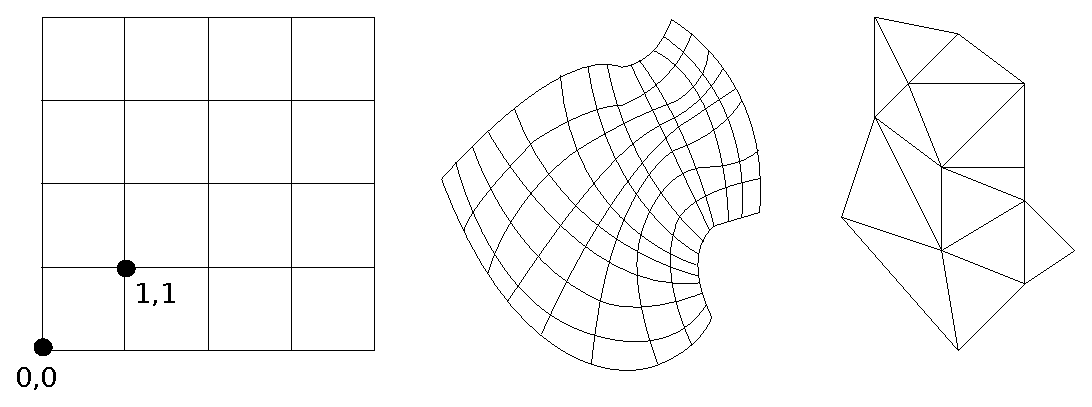
\includegraphics{./images/maillages.pdf}}
  \caption{From left to right, Cartesian, curvilinear and unstructured meshes.}
  \label{fig:mesh1}
\end{center}\end{figure}
%\begin{mydef}
%The dimension of a mesh $\mathcal{M}=(V,E)$ applied onto $\Omega=\mathbb{R}^n$ is denoted $dim(\mathcal{M})=n$.
%\end{mydef}
A mesh can be structured (as Cartesian or curvilinear meshes), unstructured, regular or irregular (without the same topology for each element) as illustrated in Figure~\ref{fig:mesh1}. 
%One can notice that more than one type of mesh is possible inside a single simulation. For example, an hybrid mesh can be defined as an unstructured mesh composed itself of a Cartesian mesh inside each of its vertices. However, in this paper single mesh simulations are addressed.

\medskip

\begin{mydefs}[Definitions (mesh)]
\item An \textit{entity} $\phi$ of a mesh $\mathcal{M}=(V,E)$ is defined as a subset of its vertices and edges, $\phi\subset V\cup E$.
\item A \textit{group of mesh entities} $\mathcal{G} \in \mathcal{P}(V\cup E)$ represents a set of entities of the same topology.%and the mesh of a group is denoted $mesh(\mathcal{G})$, \textit{i.e.} $\mathcal{G} \in \mathcal{P}(V\cup E) \Leftrightarrow mesh(\mathcal{G})=(V,E)$
%\CP{Pas clair pour moi}
\item The \textit{set of all groups of mesh entities} used in a simulation is denoted $\Phi$.
%\CP{Entities groups not defined! a propos, n'est pas set of entit*y* groups?}
\end{mydefs}

For example, in a 2D Cartesian mesh, an entity could be a cell, made up of four vertices and four edges.
A group of entities could contain all the cells, another would for example contain the vertical edges at the frontier between cells. Both groups would be part of $\Phi$. This example is illustrated in Figure~\ref{fig:meshbase}.
%\CP{Idem, pas top clair. Il y a des implicites !}

\medskip

\begin{mydef}
The finite sequence $T: (t_n)_{n\in\llbracket 0, T_{max} \rrbracket}$ represents the discretization of the continuous time domain $\mathcal{T}=\mathbb{R}$.
%To each discrete time-step $n\in\llbracket 0, T_{max} \rrbracket$, a time value $t_n\in\mathcal{T}$ is associated. The time step for $t_n$ is equal to $t_n-t_{n-1}$.
\end{mydef}

The time discretization can be as simple as a constant time-step with a fixed number of steps.
The time-step and the number of steps can also change on the fly during execution. %the simulation depending on variables values (see definitions below).

\medskip

\begin{mydefs}[Definitions (quantity)]
\item $\Delta$ are the \textit{mesh variables}. A mesh variable $\delta \in \Delta$ associates to each couple entity and time-step a value $\delta: \mathcal{G}\times T\mapsto \mathcal{V}_\delta$ where $\mathcal{V}_{\delta}$ is a value type.
\item The group of entities a variable is mapped on is denoted $entity(\delta)=\mathcal{G}$.%\CP{Pas clair}
\item $\mathcal{S}$ are the \textit{scalar variables}. A scalar variable $s \in \mathcal{S}$ associates to each time-step a value $s: T\mapsto \mathcal{V}_\delta$ where $\mathcal{V}_{\delta}$ is a value type.
\item $\mathbb{V}=\Delta\cup\mathcal{S}$ is the set of \emph{variables} or \emph{quantities}.
\item Among the scalar variables is one specific boolean variable $conv\in\mathcal{S}$, the convergence criteria, whose value is $0$ except at the last step where it is 1. This scalar can be updated on the fly according to other variables, typically by using a reduction as detailed later.%Thus, $\forall t\in \llbracket 0, T_{max-1} \rrbracket$, $conv(t)=0$, and $conv(T_{max})=1$. This makes it possible to compute while not knowing $T_{max}$ \textit{a priori}.
%\CP{Il y a des implicites : est ce un calcul jusqu'à convergence ou un calcul sur MAX time step? Ou veux tu modéliser les deux (suivant que MAX est connu a priori ou a postiori?}
\end{mydefs}
%\medskip
%
%This section has presented the formalism of meshes, their associated entities, groups of entities as well as time discretization and quantities (mapped on meshes or scalars).

%-----------------------
\subsection{Computations}

\medskip
\begin{mydefs}
\item A computation domain $D$ is a subpart of a group of mesh entities, $D \subseteq \mathcal{G} \in \Phi$.
\item The set of computation domains of a numerical simulation is denoted $\mathcal{D}$.
\item $\mathcal{N}$ is the set of neighborhood functions $n: \mathcal{G}_i \mapsto \mathcal{G}_j^m$ which for a given entity $\phi \in \mathcal{G}_i$ returns a set of $m$ entities in $\mathcal{G}_j$. One can notice that $i = j$ is possible. Most of the time, such a neighborhood is called a \emph{stencil shape}.
\end{mydefs}

\begin{mydef}
A computation kernel $k$ of a numerical simulation is defined as $k=(S,R,(w,D),comp)$, where
\begin{itemize}
\item $S \in \mathcal{S}$ is the set of scalar to read,
\item $w \in \mathbb{V}$ is the single quantity (variable) modified by the computation kernel,
\item $D$ is the computation domain on which $w$ is computed, $D \subseteq entity(w)$, or is $null$ if $w \in \Delta$,
\item $R \in \Delta \times \mathcal{N}$ is the set of tuples $(r,n)$ representing the data read where $r$ is a mesh variable read by the kernel to compute $w$, and $n : entity(w) \rightarrow entity(r)^m$ is a neighborhood function that indicates which entity of $r$ are read to compute $w$.
\item Finally, $comp$ is the numerical computation which returns a value from a set of $n$ input values, $comp: \mathcal{V}_i^n \rightarrow \mathcal{V}_j$, where $\mathcal{V}_i$ and $\mathcal{V}_j$ are value types. Thus, $comp$ represents the actual numerical expression  computed by a kernel.
\end{itemize}
\end{mydef}

In a Multi-Stencil simulation, at each time-step, a set of computations is performed. During a computation kernel, it can be considered that a set of old states ($t-1$) of quantities are read ($\mathcal{S}$ and $R$), and that a new state ($t$) of a single quantity is written ($w$).
Such a definition of a computation kernel covers a large panel of different computations. For example, the four usual types of computations (stencil, local, boundary and reduction) performed into a simulation can be defined as follow :
\begin{itemize}
\item A computation kernel $k(S,R,(w,D),comp)$ is a \emph{stencil kernel} if $\exists (r,n) \in R$ such that $n \neq identity$. %That is, if the neighborhood it accesses is not reduced to the exact point it modifies.
\item A \emph{boundary kernel} is a kernel $k(S,R,(w,D),comp)$ where $D$ is a specific computation domain at the border of entities, and which does not intersect with any other computation domain.
\item A computation kernel $k(S,R,(w,D),comp)$ is a \emph{local kernel} if $\forall (r,n) \in R$, $n = identity$.
\item A computation kernel $k(S,R,(w,D),comp)$ is a \emph{reduction kernel} if $w$ is a scalar. A reduction can for example be used to compute the convergence criteria of the time loop of the simulation.
\end{itemize}

Since we only consider explicit numerical schemes in this paper, a kernel cannot write the same quantity it reads, except locally, \textit{i.e.} if $\exists (w,n)$ where $w \in R\Rightarrow n=identity$.

It could seem counter-intuitive to restrict kernels to the computation of a single quantity.
As a matter of fact, one often performs multiple computations in a single loop, for example for performance reasons (cache optimization, temporary computation factorization, etc.) or for readability (code length, semantically close computations, etc.).
One can however notice that it is always possible to re-express a computation modifying $n$ quantities as $n$ computations modifying a single quantity each.
Both approaches are therefore equivalent from an expressiveness point of view.

%JB: l'argument me semble un peu specieux, en math on peut faire $(x,y,z) = ...$
% The definition used above actually follows the usual "=" meaning of an equation or a numerical computation, where a single variable is written on the left of the symbol.
% \item First, we think this notation is more natural for a numerician who usually manipulate equations.

Modifying multiple quantities in a single loop nest does however not always improve performance.
For example, it reduces the number of concurrent tasks available and limits the potential efficiency on parallel resources as will be shown in Section~\ref{sect:eval}.
We therefore introduce the concept of \emph{fusion} in Section~\ref{sect:parallelism} where multiple logical kernels can be executed in a single loop nest that modifies multiple quantities.
This transformation is much easier to implement than splitting a kernel would be, leaving more execution choices open.

In addition, the modification of multiple quantities in a single loop nest can lead to subtle ordering errors when executing in parallel as it will be discussed in Section~\ref{sect:fusion}.
Automatically detecting kernels that can be fused instead of leaving this to the responsibility of the domain scientist avoids these potential errors.
We have therefore chosen to restrict kernels to the computation of a single quantity.

%\JB{je garderais la discussion sur le scatter pour plus tard}
%\JB{Moreover, one can note that the usual \emph{scatter} optimization of numerical codes is actually a specific case of fusion.}

\begin{mydef}
The set of $n$ ordered computation kernels of a numerical simulation is denoted $\Gamma = [k_i]_{0 \leq i \leq n-1}$, such that $\forall k_i,k_j \in \Gamma$, if $i < j$, then $k_i$ is computed before $k_j$.
\end{mydef}

\begin{mydef}
A \textit{multi-stencil program} is defined by the octuplet 
\begin{equation}
\mathcal{MSP}(\mathcal{M},\Phi,\mathcal{D},\mathcal{N},\Delta, \mathcal{S},T,\Gamma)
\label{eq:msp}
\end{equation}
\end{mydef}

\paragraph{\textbf{Example}}
\begin{figure}[ht]
\begin{center}
\subfloat[On the left a mesh is represented, on the right two examples of groups of mesh entities are represented: cells and vertical edges.\label{fig:meshbase}]{
\resizebox{8cm}{!}{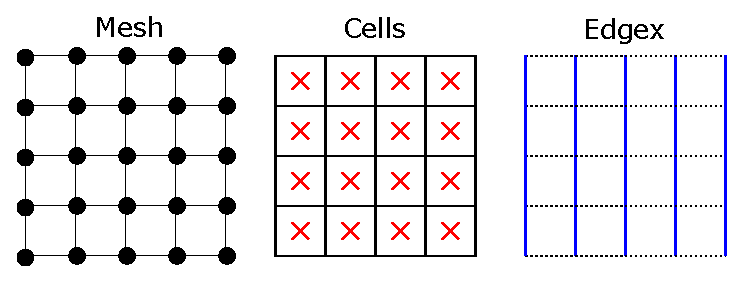
\includegraphics{./images/mesh.pdf}}
}\\
\hspace{10pt}
\subfloat[A is computed with a 4-neighborhood stencil applied on B. A is computed onto a computation domain which does not include all entities of the group.\label{fig:ex1}]{
\resizebox{5cm}{!}{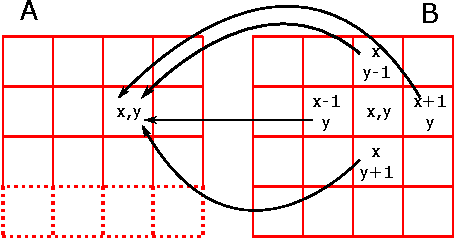
\includegraphics{./images/stencil1.pdf}}
}
\vspace{20pt}
\hspace{10 pt}
\subfloat[A is computed with a 2-neighborhood stencil applied on C. A is computed onto a computation domain includes all entities of the group.\label{fig:ex2}]{
\resizebox{5cm}{!}{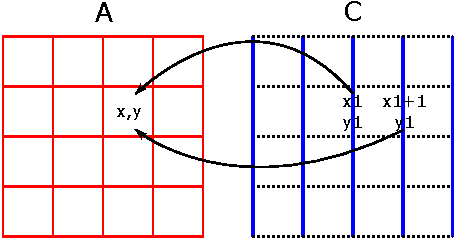
\includegraphics{./images/stencil2.pdf}}
}
\end{center}
\caption{(a) a Cartesian mesh and two kind of groups of mesh entities, (b) an example of stencil kernel on cells, (c) an example of stencil kernel on two different groups of mesh entities.}
\label{fig:gspmsp}
\end{figure}
For example, in Figure~\ref{fig:ex1}, assuming that the computation domain (full lines) is denoted $dc1$ and the stencil shape described by the neighborhood function is $n1$, the stencil kernel can be defined as:
\begin{equation*}
R: \{(B,n1)\}, \quad w: A, \quad D: dc1,
\end{equation*}
\begin{equation*}
comp: A(x,y)=B(x+1,y)+B(x-1,y)+B(x,y+1)+B(x,y-1).
\end{equation*}
On the other hand, in the example of Figure~\ref{fig:ex2}, assuming the computation domain is $dc2$ and the stencil shape is $n2$, the stencil kernel is defined as:
\begin{equation*}
R: \{(C,n2),(A,identity)\}, \quad w: A, \quad D: dc2,
\end{equation*}
\begin{equation*}
comp: A(x,y)=A(x,y)+C(x1,y1)+C(x1+1,y1).
\end{equation*}

In this section, we have formally defined a stencil program. This formalism is mainly composed of a mesh abstraction and a simple definition of computation. In fact, this formalism is generic enough to be common to many existing modelizations of a stencil computation or a stencil simulation. Thus, the formalism summarized by Equation (\ref{eq:msp}) can be compared to a meta-model of a multi-stencil program. In the next section, we use this meta-model (or meta-formalism) to define both a the domain specific language MSL, and the generic assembly of a multi-stencil program GA.
%\JB{Plusieurs fois tu parles de meta-modele... C'est un peu different de la definition communement accepte plus orientee UML de meta-modele. Heureusement que le relecteur est pas de cette communautee :)}

%Finally, one can note that the meta-formalism is independent from the topology of the mesh. This property will be kept in the rest of this paper so that MSF has the capacity to be used for any kind of mesh, thus being mesh-agnostic.
